\documentclass[../main.tex]{subfiles}

\begin{document}
	\newcommand{\T}[1]{T^{(#1)}(s)}
	
	\section{Algebra dei blocchi}
		L'algebra dei blocchi permette di calcolare la funzione di trasferimento $ T(s) $ totale di un sistema costituito dall'interconnessione di pi\'u sistemi.
		
		Solitamente la risposta forzata di un generico sistema MIMO \'e: $ \underline{y} = T \underline{u} $. L'algebra dei blocchi consiste nel considerare tutte le variabili in gioco $ (\underline{y}, T, \underline{u}) $ come scalari e operare su di essi come se fossero quantit\'a scalari. Grazie a passaggi algebrici classici, quindi si pu\'o ottenere facilmente la funzione di trasferimento totale. 
	
	\section{Risposta forzata di sistemi interconnessi}
		La connessione tra pi\'u sistemi produce un nuovo sistema caratterizzato da:
		\begin{itemize}
			\item 
				ingressi: $ \quad \underline{u}(t) = \left[ 
				\begin{smallmatrix} 
					u_1(t)
					\\
					\vdots
					\\
					u_{n_u}(t)
				\end{smallmatrix} \right] $
			\item 
				uscite: $ \quad \underline{y}(t) = \left[ 
				\begin{smallmatrix}
					y_1(t)
					\\
					\vdots
					\\
					y_{n_y}(t)
				\end{smallmatrix} \right] $
			\item 
				$ T_{ij}(s) = T_{y_i u_j}(s) \quad $ funzione di trasferimento tra l'ingresso $ u_j $ e l'uscita $ y_i $
		\end{itemize}
		Quindi un sistema MIMO non sar\'a caratterizzato da una sola funzione di trasferimento, ma da una \textbf{matrice di trasferimento}:
		\[
			T(s) =
			\begin{bmatrix}
				T_{11} & T_{12} & \dots & T_{1n_u} \\ 
				T_{21} & T_{22} & \cdots & \vdots \\ 
				\vdots & \vdots & \ddots & \vdots \\ 
				T_{n_y1}& T_{n_y2} & \cdots & T_{n_yn_u} 
			\end{bmatrix}
		\]
		Questa matrice ha:
		\begin{itemize}
			\item tante righe quante le uscite.
			\item tante colonne quante gli ingressi.
		\end{itemize}
		Quindi la risposta forzata del sistema si ottiene moltiplicando la matrice di trasferimento con il vettore colonna degli ingressi:
		\[ 
			\begin{bmatrix}
				y_1(t)
				\\[1em]
				\vdots
				\\[1em]
				y_{n_y}(t)
			\end{bmatrix} =
			\begin{bmatrix}
				T_{11} & T_{12} & \dots & T_{1 n_u} \\ 
				T_{21} & T_{22} & \cdots & \vdots \\ 
				\vdots & \vdots & \ddots & \vdots \\ 
				T_{n_y 1}& T_{n_y 2} & \cdots & T_{n_y n_u} 
			\end{bmatrix}
			\begin{bmatrix}
				u_1(t)
				\\[1em]
				\vdots
				\\[1em]
				u_{n_u}(t)
			\end{bmatrix}
		\]
		
	\subsection{Stabilit\'a BIBO}
	
		\begin{definition}
			Un sistema \'e stabile BIBO \textbf{se e solo se} qualsiasi ingresso limitato, allora l'uscita forzata $ y_f(t) $ \'e limitata. $ y_f(t) $ \'e un vettore che ha come elementi $ y_{f,1}(t), y_{f,2}(t), \dots, y_{f,n_y}(t) $, quindi affinch\'e sia stabile, tutte le componenti devono essere limitate.
		\end{definition}

		\paragraph{Condizioni}
		Nessuno elemento della matrice di trasferimento $ T(s) $, deve avere poli (radici del denominatore) a $ \Re \geq 0 $.
		
		\begin{mdframed}[style=Esempio]
			\paragraph{Esempio}
			\[ 
				T(s) =
				\begin{bmatrix}
					\dfrac{1}{s+1} & \dfrac{1}{s}
					\\[0.5cm]
					0 & \dfrac{1}{(s+1)^2}
				\end{bmatrix}
			\]
			Non \'e stabile BIBO perch\'e la componente $ T_{12}(s) $ ha un polo a $ \Re = 0 $. Infatti se poniamo un ingresso limitato: $ \underline u(t) = \left[ \begin{matrix} 0\\ \gr \end{matrix} \right] $ otteniamo un'uscita illimitata:
			\[
				Y_f(s) =
				\begin{bmatrix}
					\dfrac{1}{s+1} & \dfrac{1}{s}
					\\[1em]
					0 & \dfrac{1}{(s+1)^2}
				\end{bmatrix}
				\begin{bmatrix}
					0 
					\\[1.5em]
					\dfrac{1}{s}
				\end{bmatrix} =
				\begin{bmatrix}
					\dfrac{1}{s^2}
					\\[1em]
					\dfrac{1}{s(s+1)^2}
				\end{bmatrix}
			\]
			\begin{itemize}
				\item 
					$ \dfrac{1}{s^2} $ nel tempo corrisponde a una rampa (illimitata);
				\item
					$ \dfrac{1}{s(s+1)^2} $ nel tempo corrisponde a un gradino e a un esponenziale decrescente (limitata).
			\end{itemize}
		\end{mdframed}

	\section{Interconnessione di sistemi SISO}
		Dati due sistemi:
		\begin{itemize}
			\item 
				$ S^{(1)} $: $ \quad Y_f^{(1)}(s) = T^{(1)}(s)U^{(1)}(s) $
			\item 
				$ S^{(2)} $: $ \quad Y_f^{(2)}(s) = T^{(2)}(s)U^{(2)}(s) $
		\end{itemize}
		
	\subsection{Serie}
		\begin{figure}[H]
			\begin{subfigure}{0.5\textwidth}
				\begin{align*}
					Y_f(s) = T^{(2)}(s)U^{(2)}(s) = T^{(2)}(s) T^{(1)}(s) U(s)
					\intertext{La funzione di trasferimento del sistema complessivo \'e:}
					T(s) = T^{(2)}(s) T^{(1)}(s) \qquad\qquad\qquad\qquad
					\intertext{(NB: l'ordine di questo prodotto vale anche per i sistemi MIMO che sono descritti con matrici)}
				\end{align*}
			\end{subfigure}
			\begin{subfigure}{0.4\textwidth}
				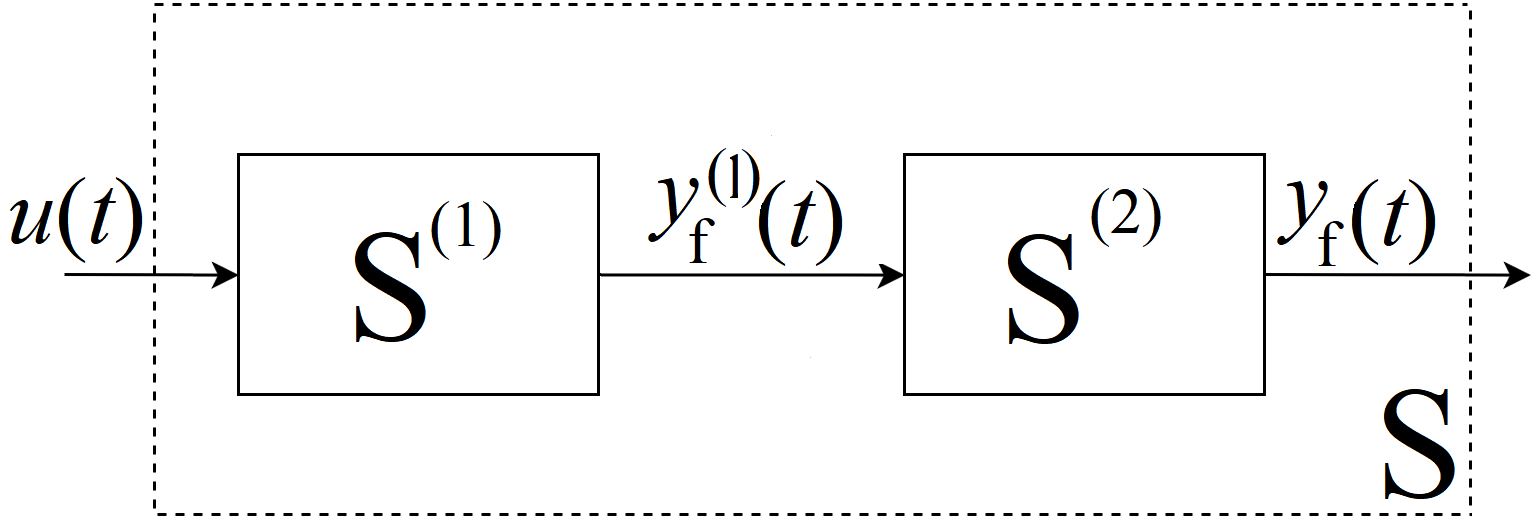
\includegraphics[width=\linewidth]{interconnections/serie}
			\end{subfigure}
		\end{figure}
		
	\subsection{Parallelo}
		\[
			Y_f(s) = T^{(1)}(s)U^{(1)}(s) + T^{(2)}(s)U^{(2)}(s) = \left[ T^{(1)}(s) + T^{(2)}(s) \right]
		\]
		\[
			T(s) = T^{(1)}(s) + T^{(2)}(s)
		\]
		
	\subsection{Retroazione (feedback)}
		\[
			y= \T{1}e = \T{1}(u-v) = \T{1}[u-\T{2}y] = \T{1}u - \T{1}\T{2}y \]
		\[ 
			[1+\T{1}\T{2}]\ y = \T{1}u \]
		\[ 
			\begin{cases}
				\T{1} \quad \text{funzione di trasferimento in catena diretta}
				\\
				\T{2} \quad \text{funzione di trasferimento in catena inversa}
			\end{cases}
		\]
		In generale sia che $ v $ venga sottratto o sommato:
		\[
			T(s) = \frac{\T{1}}{1\pm\T{1}\T{2}}
		\]
	\subsubsection{Loop algebrici}
		Se tutte le funzioni di trasferimento sono semplicemente proprie, allora si forma un \textbf{loop algebrico}, che rende irrealizzabile la retroazione.
		
		\begin{mdframed}[style=Esempio]
			\paragraph{Esempio}
			Entrambe le funzioni di trasferimento sono amplificatori e $ u(t) = 0 $, $ e(t) =1 $.
			
			\begin{figure}[H]
				\centering
				\includegraphics[width=0.4\textwidth]{interconnections/loop_algebrico}
			\end{figure}
		
			Sostituendo i valori e percorrendo la retroazione troveremo che $ e $ dovrebbe valere contemporaneamente $ 1 $ e $ -8 $. Infatti $ y $ dipende istantaneamente da $ e $, $ v $ d. i. da $ y $, $ e $ d. i. da $ v $, quindi otteniamo che $ e $ dipende istantaneamente da s\'e stessa, ovvero c'\'e un loop algebrico.
		\end{mdframed}
	
		\begin{mdframed}[style=Esempio]
			\paragraph{Esempio}
			\begin{wrapfigure}{R}{.5\linewidth}%
				\centering
				\includegraphics[width=\linewidth]{interconnections/esempio_retroazione}%
			\end{wrapfigure}
			\leavevmode%
			\'E possibile trovare $ k $ per avere un sistema stabile BIBO?\\
			Notiamo subito che non ci sono loop algebrici perch\'e non tutte le funzioni di trasferimento sono semplicemente proprie. Pertanto la funzione di trasferimento \'e:
			\[
				T(s) = \dfrac{\dfrac{1}{s^2+1}}{1 + \dfrac{k}{s^2+1}} =
				\dfrac{\dfrac{1}{s^2+1}}{\dfrac{s^2+1+k}{s^2+1}} = 
				\dfrac{1}{s^2+1+k}
			\]
			\[ 
				s^2 = -(k+1)
			\]
			Affinch\'e il sistema sia stabile BIBO, non ci devono essere radici a $ \Re \geq 0 $
			\begin{itemize}
				\item 
					$ k<-1 \quad \Rightarrow \quad s_{1,2} = \pm \sqrt{-(k+1)} $
				\item
					$ k>-1 \quad \Rightarrow \quad s_{1,2} = \pm j \sqrt{k+1} $
				\item 
					$ k=-1 \quad \Rightarrow \quad s_{1,2} = 0 $
			\end{itemize}
			Non esiste alcun $ k $ per cui il sistema sia stabile BIBO.
		\end{mdframed}

		%esercizi
		\documentclass[../main.tex]{subfiles}

\begin{document}
	\section{Esercizio}
	Calcolare tutte le possibili funzioni di trasferimento del sistema:
	\begin{figure}[h!]
		\centering
		\begin{subfigure}{0.8\textwidth}
			\includegraphics[width=\textwidth]{interconnections/algebra_blocchi_es1_1}
		\end{subfigure}%
	\end{figure}
	\begin{itemize}
		\item $ T_{y_1 u_1}(s) $: poniamo $ u_2 = 0 $.\\
		\parbox[t]{\dimexpr\textwidth-\leftmargin}{%
			\vspace{-2.5mm}
			\begin{wrapfigure}{r}{0.5\textwidth}
				\centering
				\vspace{-\baselineskip}
				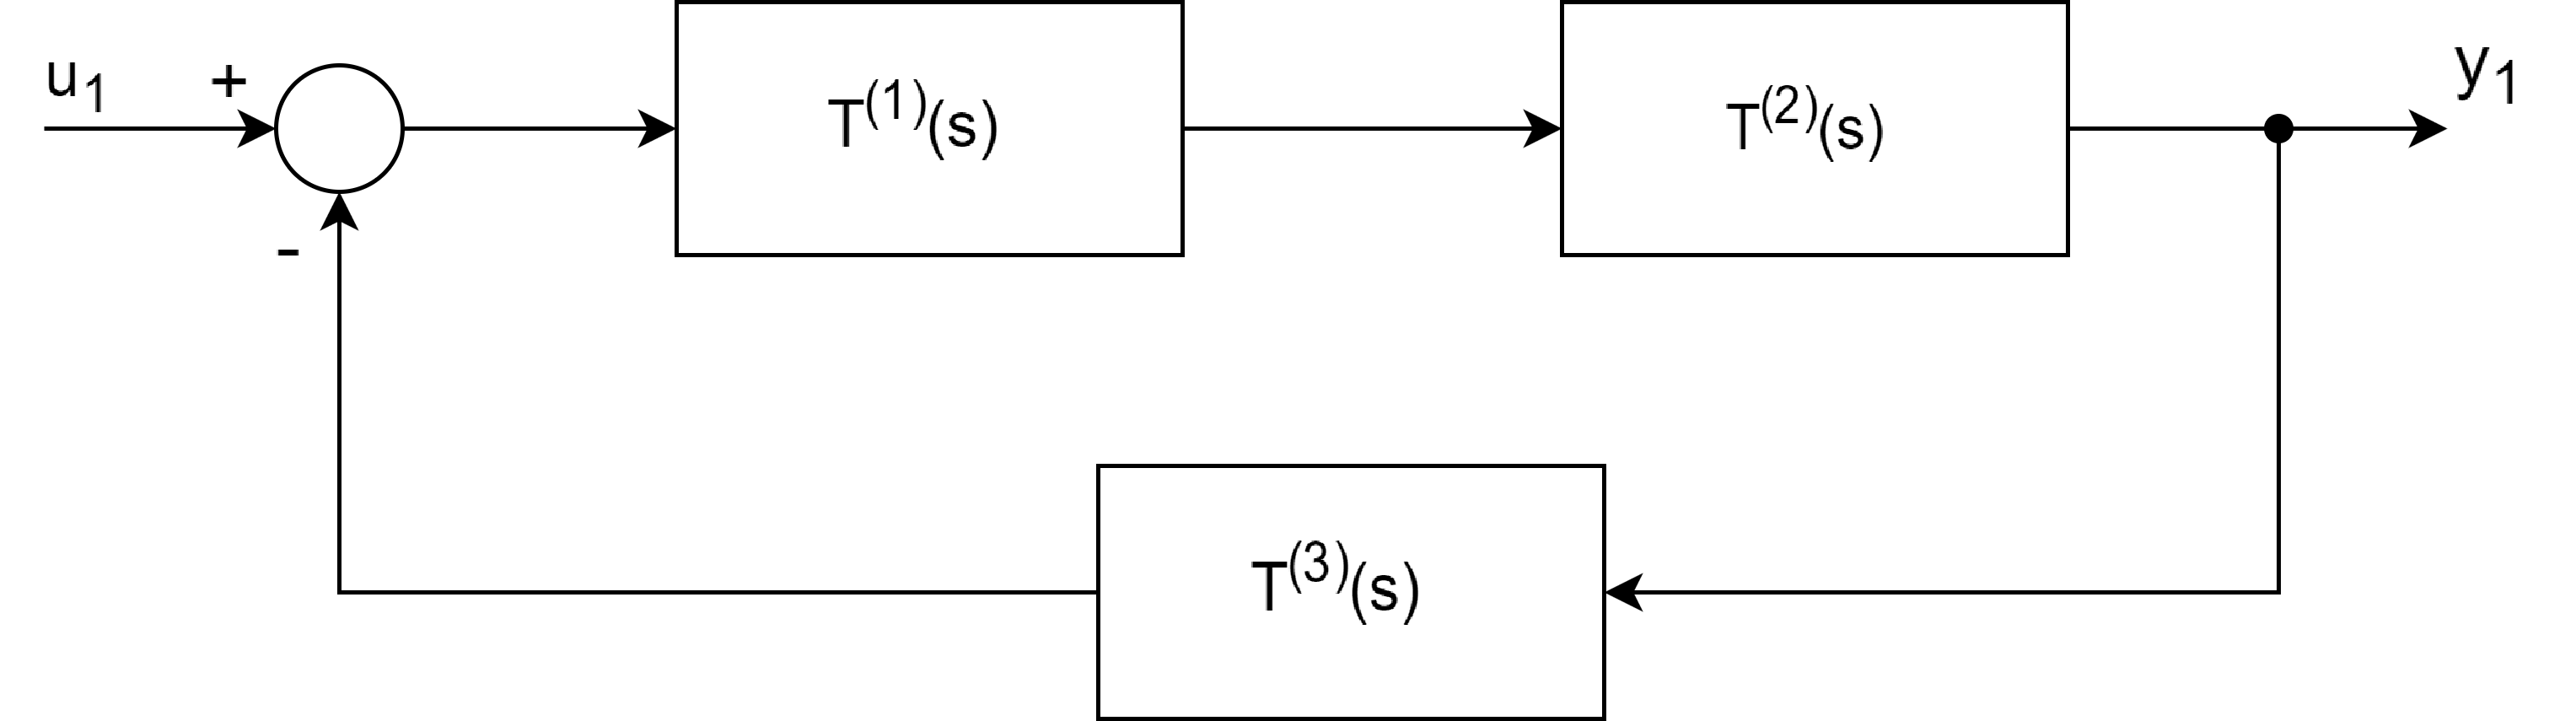
\includegraphics[width=\linewidth]{interconnections/algebra_blocchi_es1_2}
			\end{wrapfigure}
			Serie tra $ T^{(1)} $ e $ T^{(2)} $:
			\[ T_{serie} = T^{(1)} T^{(2)} = \frac{s+1}{s-1} \frac{1}{s+1} = \frac{1}{s-1} \]
			Retroazione tra $ T_{serie} $ e $ T^{(3)} $:
			\[ T_{y_1 u_1}(s) = \frac{T_{serie}}{1+T_{serie} T^{(3)}} = \frac{\frac{1}{s-1}}{1+\frac{1}{(s+1)(s-1)}} = \frac{\frac{1}{s-1}}{\frac{1}{(s^2-1+1)(s-1)}} = \frac{s+1}{s^2} \]
			Questa funzione di trasferimento \'e instabile BIBO perch\'e c'\'e un polo a $ \Re = 0 $.
		}
		%
		\item $ T_{y_1 u_2}(s) $: poniamo $ u_1 = 0 $.\\
		\parbox[t]{\dimexpr\textwidth-\leftmargin}{%
			\vspace{-2.5mm}
			\begin{wrapfigure}[10]{r}{0.5\textwidth}
				\centering
				\vspace{-\baselineskip}
				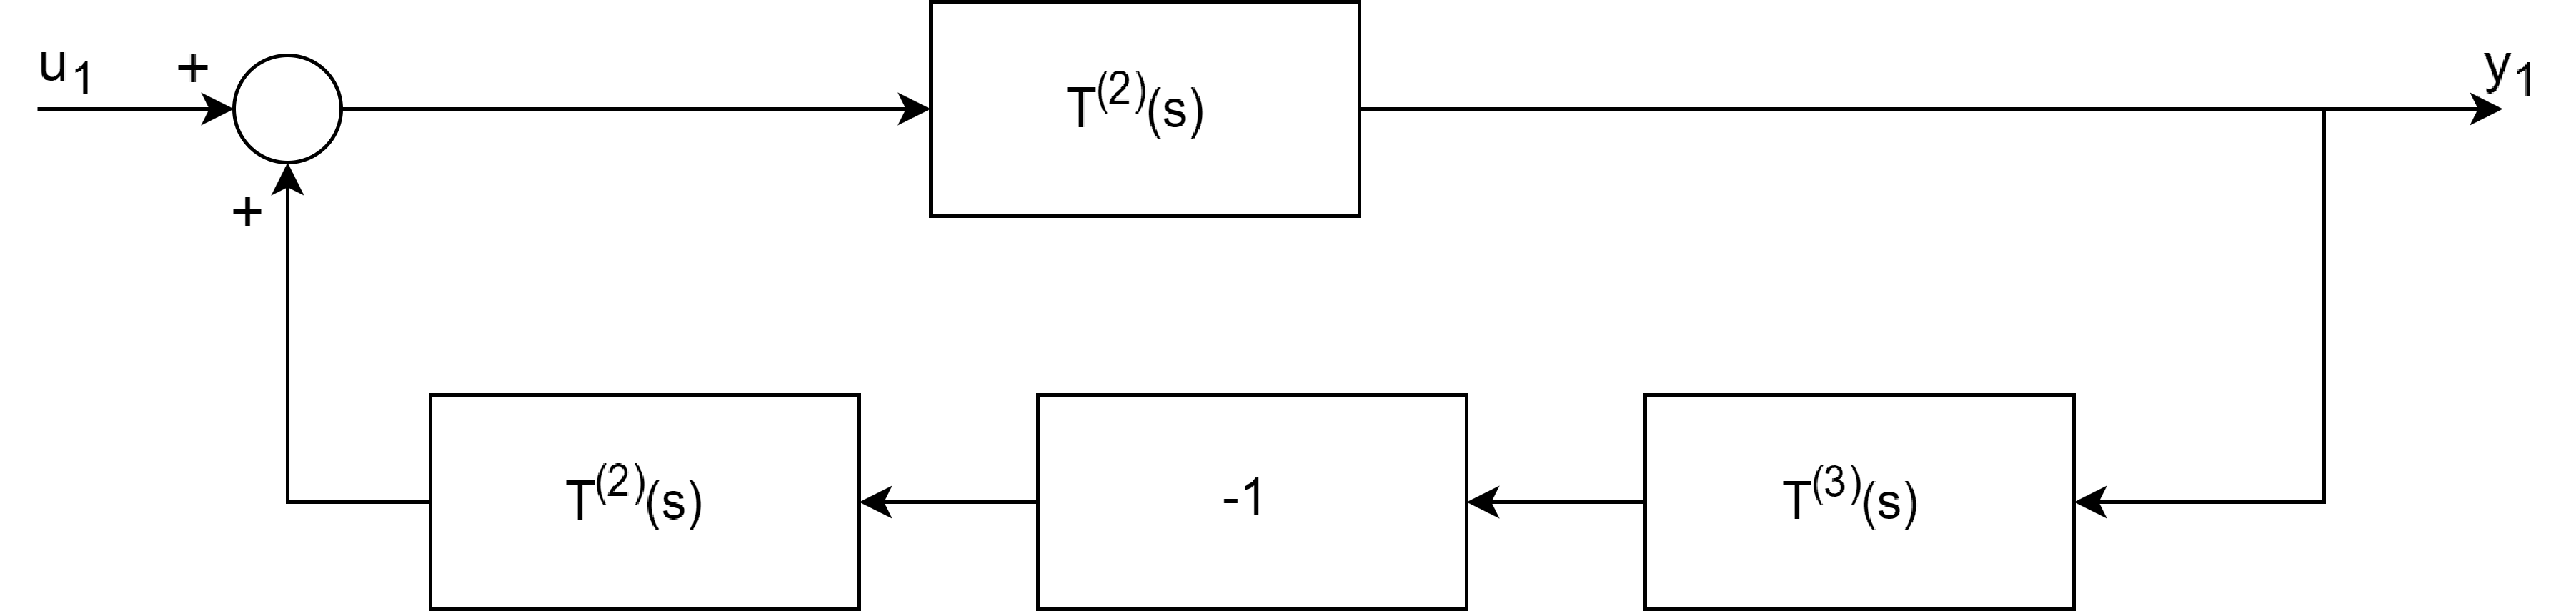
\includegraphics[width=\linewidth]{interconnections/algebra_blocchi_es1_3}
			\end{wrapfigure}
			Calcoliamo la serie nella catena inversa di retroazione:
			\[ T_{serie}(s) = \frac{-1}{(s+1)^2} \]
			Retroazione:
			\[ T_{y_1 u_2}(s) = \frac{\frac{s+1}{s-1}}{1-\frac{s+1}{s-1}\frac{-1}{(s+1)^2}} = \frac{\frac{s+1}{s-1}}{1+\frac{1}{(s+1)(s-1)}} = \frac{\frac{s+1}{s-1}}{\frac{s^2}{(s+1)(s-1)}} = \frac{(s+1)^2}{s^2} \]
			Questa funzione di trasferimento \'e instabile BIBO perch\'e c'\'e un polo a $ \Re = 0 $.
			Abbiamo ottenuto una funzione di trasferimento semplicemente propria perch\'e tra $ u_2 $ e $ y_1 $ in catena diretta c'\'e una dipendenza istantanea (dato dalla costante):
			\[ T^{(2)}(s) = \frac{s+1}{s-1} = 1 + \frac{2}{s-1} \]
		}
		%
		\item $ T_{y_2 u_1}(s) $:
		\[ T_{y_2 u_1}(s) = \frac{\frac{s+1}{s-1}\frac{1}{s+1}}{1+\frac{s^2}{(s+1)(s-1)}} = \frac{1}{s^2} \]
		%
		\item $ T_{y_2 u_2}(s) $:
		\[ T_{y_2 u_2}(s) = \frac{\frac{1}{s-1}}{\frac{s^2}{(s+1)(s-1)}} = \frac{s+1}{s^2}\]
	\end{itemize}
	%
	\section{Esercizio}
	Calcolare la funzione di trasferimento del sistema in figura:
	\begin{center}
		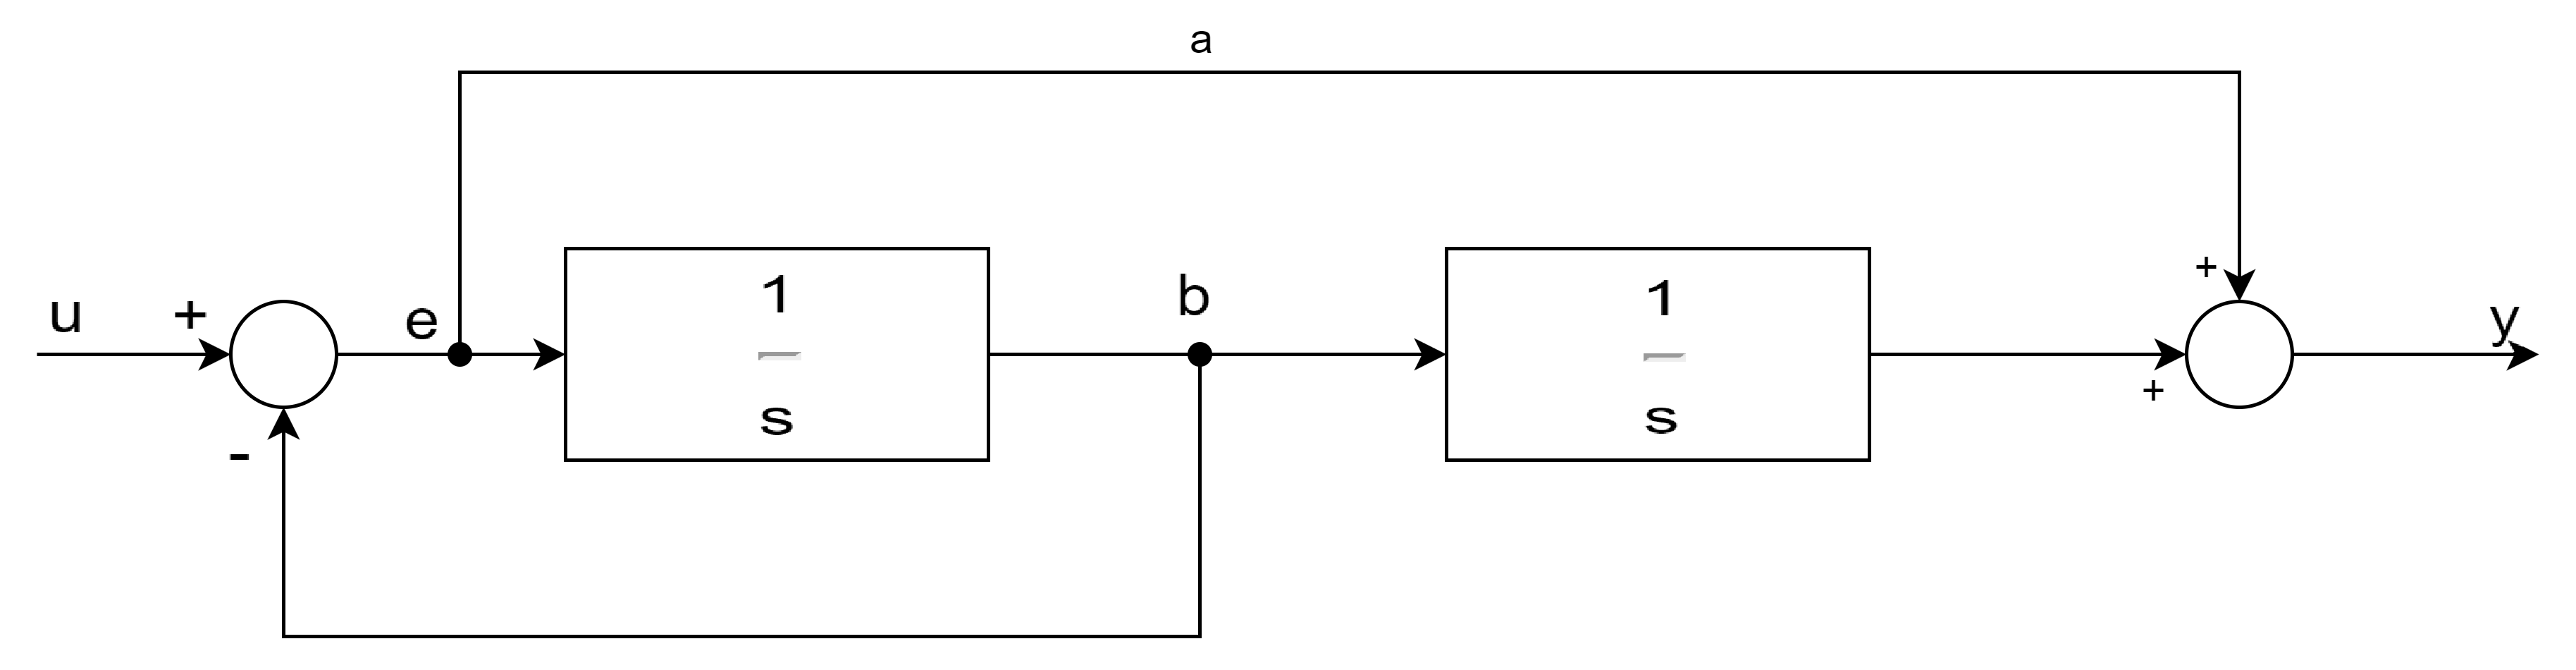
\includegraphics[width=\textwidth]{interconnections/algebra_blocchi_es2_1}
	\end{center}
	Spostiamo il nodo $ e $ e otteniamo un nuovo sistema composto da una retroazione e da un parallelo.\\
	L'algebra dei blocchi permette di fare queste equivalenze solo per il calcolo della funzione di trasferimento complessiva e non per altri calcoli, perch\'e stiamo introducendo nuovi blocchi, tra cui alcuni irrealizzabili (vedi il blocco di funzione di trasferimento $ s $).
	\begin{figure}[h!]
		\centering
		\begin{subfigure}{0.5\textwidth}
			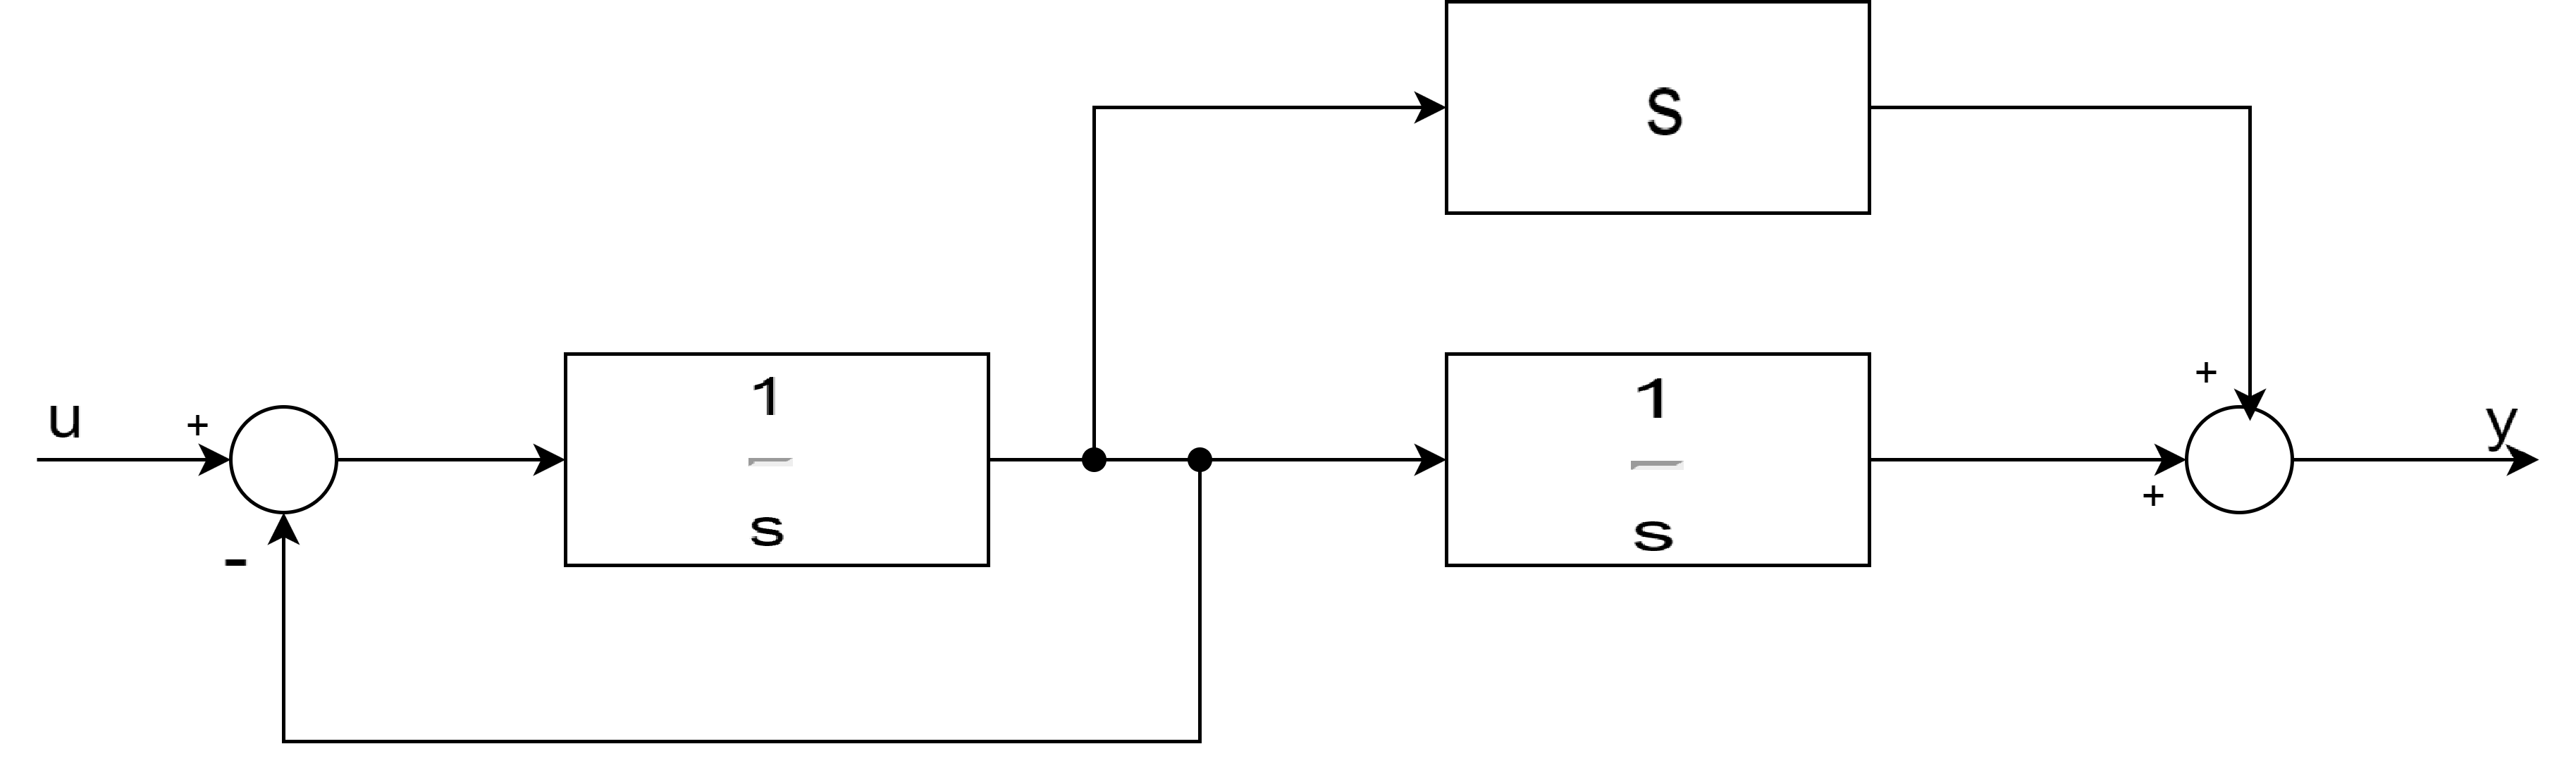
\includegraphics[width=\textwidth]{interconnections/algebra_blocchi_es2_2}
		\end{subfigure}%
		\begin{subfigure}{0.5\textwidth}
			\includegraphics[width=\textwidth]{interconnections/algebra_blocchi_es2_3}
		\end{subfigure}%
	\end{figure}
	\[ T_{yu}(s) = \frac{\frac{1}{s}}{1+\frac{1}{s}} \left( s+\frac{1}{s} \right) = \frac{s^2+1}{s(s+1)} \]
\end{document}
\end{document}